
% Document class options:
% =======================
% blind: Anonymise all author, affiliation, correspondence
%        and funding information.
%
% lineno: Adds line numbers.
%
% serif: Sets the body font to be serif. 
%
% twocolumn: Sets the body text in two-column layout. 
% 
% num-refs: Uses numerical citation and references style 
%           (Vancouver-authoryear).
%
% alpha-refs: Uses author-year citation and references style
%             (rss).
%
% Using other bibliography styles:
% =======================
%
% To specify a different bibiography style
%
% 1) Do not use either num-refs or alpha-refs in documentclass.
% 2) Load natbib package with the options set as needed.
% 3) Use the \bibliographystyle command to specify the style
% 
% Included NJD styles are: 
%   WileyNJD-ACS
%   WileyNJD-AMA
%   WileyNJD-AMS
%   WileyNJD-APA
%   WileyNJD-Harvard
%   WileyNJD-VANCOUVER
%
% or you may upload an alternative .bst file 
% (if requested by the journal).
%
% Examples:
% =======================
%% Example: Using numerical, sort-by-authors citations.
\documentclass[authordate, serif, review]{jote-article}


\usepackage{latexsym}
\usepackage[normalem]{ulem}
\usepackage{soul}
\usepackage{array}
\usepackage{extarrows}
\usepackage{graphicx}

\usepackage{subfig}
\usepackage{wrapfig}
\usepackage{enumitem}
\usepackage{adjustbox}
\usepackage{longtable}
\usepackage{changepage}
\usepackage{setspace}
\usepackage{hhline}
\usepackage{multicol}
\usepackage{tabto}
\usepackage{multirow}
\usepackage{fancyhdr}
%\usepackage[toc,page]{appendix}

\usepackage{flowchart}
%\usepackage[paperheight=11.0in,paperwidth=8.5in,left=0.5in,right=0.5in,top=1.0in,bottom=1.0in,headheight=1in]{geometry}
\usepackage[utf8]{inputenc}
\usepackage[T1]{fontenc}
\usepackage{csquotes}


%\addbibresource{julie.bib}


%% Example: Using author-year citations and anonymising submission
% \documentclass[blind,alpha-refs]{wiley-article}

%% Example: Using unsrtnat for numerical, in-sequence citations
% \documentclass{wiley-article}
% \usepackage[numbers]{natbib}
% \bibliographystyle{unsrtnat}

%% Example: Using WileyNJD-AMA reference style and superscript
%%          citations, two-column and serif fonts for AIChE
% \documentclass[serif,twocolumn,lineno]{wiley-article}
% \usepackage[super]{natbib}
% \bibliographystyle{WileyNJD-AMA}
% \makeatletter
% \renewcommand{\@biblabel}[1]{#1.}
% \makeatother

% Add additional packages here if required
\usepackage{siunitx}


\usepackage{float}
\usepackage{bookmark}
\usepackage{lipsum}
% Update article type if known
% Include section in journal if known, otherwise delete
\papertype{Empirical}

\title{Alcohol Cues and Their Effects on Sexually Aggressive Thoughts}

% List abbreviations here, if any. Please note that it is preferred that abbreviations be defined at the first instance they appear in the text, rather than creating an abbreviations list.
%\abbrevs{ABC, a black cat; DEF, doesn't ever fret; GHI, goes home immediately.}

% Include full author names and degrees, when required by the journal.
% Use the \authfn to add symbols for additional footnotes and present addresses, if any. Usually start with 1 for notes about author contributions; then continuing with 2 etc if any author has a different present address.

%Please also enter the authors in the same order here, for metadata purposes. This is a workaround.

\author[1]{Alexa Ruel} 
\author[2]{Jeremy Ullman}
%\authorfour{}
%\authorfive{}

%\contrib[\authfn{1}]{Equally contributing authors.}

% Include full affiliation details for all authors
\affil[1]{Reviewer 1}
\affil[2]{Reviewer 2}

\ogauthor{Julie Leboeuf, Stine Linden-Anderson, Jonathan Carriere}
\prround{2}
%\affil[2]{Department, Institution, City, State or Province, Postal Code, Country}

\corraddress{Julie Leboeuf, Department of Psychology, Bishop's University, Sherbrooke, Quebec, J1M 1Z7, Canada}
\corremail{jleboeuf16@ubishops.ca}

%\presentadd[\authfn{2}]{Department, Institution, City, State or Province, Postal Code, Country}

\paperdoi{10.36850/e1}

% Include the name of the author that should appear in the running header
\runningauthor{Leboeuf et al.}

\jname{Journal of Trial and Error}
\jyear{2020}
%\jvolume{Fall}
\jwebsite{https://jtrialerror.com}
%\paperrevised{May 18th 2020}
\paperpublished{2 December, 2020}
\paperpublisheddate{2020-12-2}
%\jpages{1-12}
\jlogo{media/jote_logo_full}



%\keywords{alcohol, automatic cognition, gender stereotypes, lexical decision task, sexual aggression}

%\abstracttext{Alcohol and its effects on aggression have been the subject of many discussions and research papers. Despite this fact, there is still a debate surrounding what it is exactly about alcohol that causes aggression. The current study sought to replicate the past finding by Bartholow \& Heinz (2006), that alcohol cues without consumption increase the accessibility of aggressive thoughts, which can then influence aggressive behaviors. In the present study, participants had to complete a lexical decision task that was set up to assess whether aggressive words were detected faster in the presence of alcohol-related pictures compared to neutral pictures. The results of this study did not replicate the expected finding as only a main effect of word type was found in which participants detected neutral words faster than aggressive words. Furthermore, the study aimed to assess the role of gender stereotype acceptance levels in this association, but due to faulty design considerations, such analyses were not possible. The results are discussed in terms of the limitations of the study, and propositions for future directions are addressed.}


\heightabstract{70mm}
\widthaffil{65mm}

\setlength{\parskip}{0pt}

%\contributions{\lipsum[1]}

\keywordsabstract{alcohol, automatic cognition, gender stereotypes, lexical decision task, sexual aggression}


\begin{document}
\begin{frontmatter}
\maketitle

\begin{abstract}
%\phantomsection
%\addcontentsline{toc}{section}{Abstract}

\noindent Alcohol and its effects on aggression have been the subject of many discussions and research papers. Despite this fact, there is still a debate surrounding what it is exactly about alcohol that causes aggression. The current study sought to replicate the past finding by Bartholow and Heinz (2006) that alcohol cues without consumption increase the accessibility of aggressive thoughts, which can then influence aggressive behaviors. In the present study, participants had to complete a lexical decision task that was set up to assess whether aggressive words were detected faster in the presence of alcohol-related pictures compared to neutral pictures. The results of this study did not replicate the expected finding as only a main effect of word type was found in which participants detected neutral words faster than aggressive words. Furthermore, the study aimed to assess the role of gender stereotype acceptance levels in this association, but due to faulty design considerations, such analyses were not possible. The results are discussed in terms of the limitations of the study, and propositions for future directions are addressed. 

% Please include a maximum of seven keywords
\end{abstract}
\end{frontmatter}

\begin{multicols}{2}
\phantomsection
\addcontentsline{toc}{section}{Take Home Message}
\section*{Take Home Message} \gotoreview
\label{sec:take-home}

\noindent  The present study failed to replicate the finding by Bartholow and Heinz (2006) that alcohol cues without consumption increase the accessibility of aggressive thoughts. This failure to replicate can be partly explained by a flawed sample; the small sample size reduced statistical power, and the different composition of the sample compared to the original study impacted the ability to recreate the results. Furthermore, some important methodological flaws concerning the choices of stimuli, particularly with regards to sexually aggressive words and neutral pictures, seriously reduced the quality of the material. Overall, poor design considerations most likely account for the failure to replicate.

\phantomsection
\addcontentsline{toc}{section}{Introduction}
\section*{Introduction} \gotoreview
\label{sec:introduction}

\noindent According to the World Health Organization (2018), harmful use of alcohol results in 3 million deaths worldwide every year. Furthermore, Field, Caetano, and Nelson (2004) found that among all the factors under investigation, what appeared to be the strongest predictor of intimate partner violence was the expectations of aggressive behavior following alcohol consumption. Although the pharmacological effects of alcohol have been well researched (Chermack \& Taylor, 1995; Giancola, 2000; Heinz, Beck, Meyer-Lindenberg, Sterzer, \& Heinz, 2001), there is less information available with regards to other factors, such as cognition and expectancies, that can lead to aggression in alcohol-related contexts. Bartholow and Heinz (2006) as well as Subra, Muller, B\`{e}gue, Bushman, and Delmas (2010) researched whether simple exposure to alcohol-related cues unconsciously increases the availability of aggressive thoughts, thus increasing the possibility of subsequent aggressive behaviors. In both studies, the researchers found that participants made faster lexical decisions when aggression-related words were paired with alcohol-related pictures compared with neutral primes. 

Before exploring more thoroughly the body of research pertaining to automatic aggressive cognition associated with a sheer exposure to alcohol cues, it is worthwhile to mention that similar studies have examined how other stimuli can generate aggressive thoughts. In 1998, Anderson, Benjamin, and Bartholow reported that simple identification of weapon primes was linked to an increase in aggressive thoughts. In this study, participants named aggressive words faster compared with nonaggressive words when presented with a weapon prime. The authors argued that this increase resulted from the weapon stimuli automatically priming aggression-related thoughts (1998). More specifically, Anderson and colleagues referred to the semantic network model of memory which posits that words or concepts that are similar in meaning or that repeatedly co-occur together are activated simultaneously in the semantic memory and therefore develop strong associations. This model goes as far as to propose that this increase in aggressive thoughts subsequently increases the likelihood that these thoughts will affect behavior (Bartholow \& Heinz, 2006).

While weapons have been reported to be linked with an increase in aggression-related thoughts, other elements from the environment that could similarly influence levels of aggressive thoughts, such as alcohol, should also be considered. Although it is generally accepted that alcohol increases aggression, there is still a debate as to what precisely causes or explains this increase (Bartholow \& Heinz, 2006), and it is usually best explained through a combination of theories and viewpoints (see Heinz et al., 2001 for a comprehensive review). Some leading theories include the \textit{physiological disinhibition} hypothesis, the \textit{indirect cause} hypothesis, and the \textit{expectancy }hypothesis (Bushman, 2002). Briefly stated, the \textit{physiological disinhibition} hypothesis states that alcohol intake increases the levels of aggression by anesthetizing the part of our brain that usually keeps our aggressive impulses under control, making people more likely to express aggressive behaviors (2002). Following a similar line of reasoning, the \textit{indirect cause} explanation proposes that alcohol consumption might increase aggression tendencies by producing changes at the cognitive and emotional levels, such as by affecting intellectual functioning and reducing self-awareness, which then increases the likelihood of aggressive acts being committed. (2002). As for the \textit{expectancy }hypothesis, it holds that alcohol is linked with aggression because people expect it to be that way (2002). This presumed effect/expectancy hypothesis suggests that people tend to associate aggression and alcohol together, even if only unconscious, which potentially accounts for one of the ways in which alcohol intake is linked with aggression (Batholow \& Heinz, 2006). The problem with this hypothesis is that evidence supporting it mostly comes from placebo designs, which makes it is unclear whether a belief that alcohol consumption has occurred is necessary for this unconscious association to be activated, or whether the presence of alcohol cues alone can increase the accessibility of aggressive thoughts (2006). 

To address this methodological limitation, Bartholow and Heinz (2006) conducted a study in which they examined the extent to which alcohol cues without consumption or belief that alcohol has been consumed (i.e., placebo effect) could increase the accessibility of aggressive thoughts. They tested 121 undergraduate students and had them participate in a lexical decision task. The participants were first primed with a stimulus and were then shown a string of letters, and they had to decide whether the letter string presented to them was a legitimate English word. The priming stimuli could either be alcohol-related pictures, weapon-related pictures, or neutral images, and the letter strings could either represent aggression-related words, neutral words, or nonwords. In this experiment, the neutral images consisted of plants, and the weapon pictures were included to create a reference point by allowing comparison with the results showing a link between weapon exposure and aggressive thoughts obtained by Anderson, Benjamin, and Bartholow (1998). Results showed that participants identified aggression-related words faster when exposed to aggression-related pictures compared with neutral images.

In 2010, Subra and colleagues replicated the study by Bartholow and Heinz (YEAR) with a different population as well as by including a slight methodological alteration. First, their study was conducted with a French-speaking population as opposed to an English one, and the sample was not restricted to undergraduate students. Subra and his colleagues used the same stimuli as those used by the authors of the 2006 study, with the exception that they selected different images for the neutral condition. They criticized the ones previously used by Bartholow and Heinz on the basis that their nature (i.e. plants) was not neutral since nature scenes have been shown to decrease aggressive thoughts (Kuo \& Sullivan, 2001a, 2001b). Instead, they used photos displaying non-alcoholic beverages for their neutral condition. Similarly to the study under replication, participants made faster lexical decisions about aggression-related words when exposed to alcohol or weapon primes compared with neutral primes. 

The two studies by Bartholow and Heinz (2006) and Subra et al. (2010) suggest that exposure to alcohol cues without consumption is linked with an increase in aggression-related thoughts. Interestingly, the target words that were used for the aggression category were mainly of a physical nature (e.g., punch, assault, murder) and did not specifically assess sexual violence. It would be worth investigating whether this increase in thoughts of an aggressive nature also extends to sexual violence, especially when considering that the World Health Organization (n.d.) listed the use of alcohol or drugs as a factor that increases the risk of men committing rape, and that severe alcohol intoxication is implicated in almost half of all sexual aggression cases worldwide (Testa, 2002). Additionally, past research has shown that alcohol priming without consumption can increase sexual expectancies. Friedman, McCarthy, F\"{o}rster, and Denzler (2005) reported that men who were exposed to suboptimal alcohol-related words rated women as being more sexually attractive, and that this effect was more precisely caused by the sexual expectancies associated with alcohol intake. It does not seem too farfetched to assume that similar effects could be found with sexual violence. The online article ``Touch-sensitive dress reveals staggering level of sexual harassment at clubs'' provides a powerful demonstration of how severe the problem of unwanted touching and sexual aggressions is in alcohol settings such as bars and clubs. The article reports about an experiment conducted by the ad agency Ogilvy in which three women were asked to wear a touch-sensitive dress to a nightclub in Brazil. The authors recorded how many times women were touched or groped in the span of three hours and 47 minutes; the total count was 157, and the principal areas where women were being touched included the waist, buttocks and thighs (Hignett, 2018).

Another element that was not assessed in the 2006 and 2010 studies is gender stereotypes acceptance. In one study, Abbey (2002) reported that traditional gender roles beliefs about dating and sexuality could be at play in explaining the occurrence of sexual assaults, irrespective of whether alcohol was involved or not. More precisely, endorsing beliefs such as interpreting a woman's refusal as an invitation to be convinced, or that forced sex is sometimes acceptable, was a proposed factor that could increase the likelihood of sexual assaults being committed. While recognizing that this is a good first step into assessing the role of gender stereotypes acceptance with regards to sexual violence, more general gender role beliefs should be investigated to truly understand the function that gender stereotypes play in sexual violence occurrences. To this effect, Locke and Mahalik (2005) reported that men who showed a problematic use of alcohol and who conformed to such masculine norms as having power over women and being violent were more inclined to score higher on the Rape Myth Acceptance Scale and to report more sexually aggressive behaviors. The first study mentioned here only looked at gender stereotypes with regards to sexuality and dating (Abbey, 2002), and although this second study by Locke and Mahalik (2005) might seem to assess gender stereotypes more globally, it appears biased towards specific stereotypes with regards to power dynamics between men and women. Another problem with the literature on gender stereotype beliefs and its relationship to violence is that the vast majority of the articles available only report on the likelihood of men committing sexually violent behaviors, or on the relationship between men's level of gender stereotypes and the perpetration of violent acts, thus leaving women out of the picture (Jakupcak, Lisak, \& Roemer, 2005; Gidycz, Warkentin, \& Orchowski, 2007; Abbey, Clinton-Sherrod, McAuslan, Zawacki, \& Buck 2003). There is a clear need to investigate the relationship between gender stereotype beliefs and sexual violence as it relates not only to men, but to women as well. 

\phantomsection
\addcontentsline{toc}{section}{Objective and Hypotheses}
\section*{Objective and Hypotheses}

The objective of this project is to further the line of research on the effects of alcohol cues on aggressive behaviors by testing this relationship specifically with sexually aggressive words and by taking into account gender stereotype beliefs. More precisely, the aggressive words used by Bartholow and Heinz (2006) will be replaced by aggressive words of a sexual nature. The comparison point will be against the two studies that have investigated this before and for which significant results have been reported, namely the one by Bartholow and Heinz (2006) and the one by Subra et al. (2010). Gender stereotypes acceptance will be evaluated through the German Extended Personal Attributes Questionnaire (Runge, Frey, Gollwitzer, Helmreich, \& Spence, 1981).

Alcohol intoxication is associated with high levels of both physical violence (Lipsey, Wilson, Cohen, \& Derzon, 2002) and sexual violence (World Health Organization, n.d.). To the current knowledge of the first author, there is no obvious reason to believe that the association between sexually aggressive words and alcohol primes should be any different than that observed between physically aggressive words and alcohol primes. Thus, it is hypothesized that participants will make faster lexical decisions to aggressive words of a sexual nature when paired with alcohol-related primes compared with neutral primes. A similar effect should also be found with the weapon-related primes. Furthermore, it is suggested that for both men and women this association will likely be different depending on one's level of gender stereotypes acceptance. Indeed, results are expected to show a non-significant association at low levels of gender stereotypes beliefs, a moderate interaction at medium levels of gender stereotype beliefs, and a dramatically significant interaction at high levels of gender stereotype beliefs. Finally, for replication purposes, it is expected that participants will be slightly more accurate at identifying neutral words compared with aggressive words. 

\label{sec:methods}
\phantomsection
\addcontentsline{toc}{section}{Methods}
\section*{Methods} \gotoreview
\phantomsection
\addcontentsline{toc}{subsection}{Participants}
\subsection*{Participants}
Sixty participants took part in this study, but two of them were excluded from the analyses, giving a final sample size of 58. One participant was excluded because the experiment failed before the data could be recorded, and the other participant was excluded because it was clear from the debriefing session that this participant had not understood the computer task properly. Furthermore, this participant's accuracy rate was only 68.54\% compared with a mean accuracy rate of 95.08\% (\textit{SD }= 4.62) for the sample. On this distribution, a score of 68.54\% represents a z-score of -5.74, providing sufficient grounds for excluding the data from the analyses. 

From the remaining participants, 49 self-identified as women (84.5\%) and nine as men (15.5\%). No one expressed a mismatch between their sex at birth and gender identified with, and no one selected the `other' option for their self-identified gender. The age of the participants ranged between 18 years old and 46 years old (\textit{M }= 21.64, \textit{SD }= 7.71) and they were all enrolled at Bishop's University. Different programs were represented, but most participants (\textit{n} = 38) were majoring in psychology. The other programs represented included biology (\textit{n} = 4), languages (\textit{n} = 3), education (\textit{n} = 2), sociology (\textit{n} = 2), physics (\textit{n} = 1), political sciences (\textit{n} = 1), biochemistry (\textit{n} = 1), history (\textit{n} = 1), English literature (\textit{n} = 1), mathematics (\textit{n} = 1), finance (\textit{n} = 1), arts administration (\textit{n} = 1), and sports studies (\textit{n} = 1).  

\subsection*{Stimuli and Task}
\addcontentsline{toc}{subsection}{Stimuli and Task}

\subsubsection*{Questionnaires} In this experiment two different questionnaires were used: a short demographic questionnaire (see Appendix A) and the German Extended Personal Attributes Questionnaire, a scale evaluating gender stereotype acceptance and beliefs (Runge, Frey, Gollwitzer, Helmreich, \& Spence, 1981). This questionnaire includes two subscales both comprising eight items, namely ``expressivity'' and ``instrumentality'', which are intended to measure the degree to which someone can be classified according to masculine (i.e., instrumentality subscale) or feminine (i.e., expressivity subscale) adjectives. In its original form, this questionnaire was designed to assess self-ascribed masculinity or femininity, but for the purpose of this study, it was modified to assess one's view and degree of endorsement of gender stereotypes in general (see Appendix B). However, it is likely that the original questionnaire and the way in which it should be coded were manipulated to the extent that the results were uninterpretable. For this reason, the results of the German Extended Personal Attributes Questionnaire are not reported. The related design-related issues are further explored in the Limitations section.

\subsubsection*{Task} Participants completed a lexical decision task in which they had to decide whether a string of letters presented to them was a legitimate English word. Prime stimuli consisted of fifteen photos: five containing alcohol bottles, five portraying weapons, and five showing non-alcoholic beverages (see Figure 1 for sample pictures). Target words were also divided into three categories, each containing 15 words (see Appendix C for the complete list): aggression-related words of a sexual nature (e.g., grope, rape), neutral words (e.g., observe, vanish), and nonword letter strings (e.g., wenct, jork). Each photo was paired with 3 aggressive words, 3 non-aggressive words, and 3 nonword letter strings for a total of 135 trials. For each trial, an image was presented for 300ms, followed by a 200ms interval prior to the showing of the target word, which stayed on the screen until the participants responded or up to 3 seconds. Participants had to indicate by pressing on a key whether the letters formed a legitimate English word or not. An interval of 3 seconds separated each trial.

\phantomsection
\addcontentsline{toc}{subsection}{Procedures}
\subsection*{Procedures}

Participants were asked to come to the Psychological Health and Well-Being lab on Bishop's University campus for one session lasting between 30 minutes and 45 minutes. Following the procedure by Barthlow and Heinz (2006), partial disclosure was used in that participants were told that the goal of the experiment was to measure the speed of language comprehension in the presence of distractive information (i.e., pictures). Once they had agreed to participate in the study, the participants were asked to complete two different paper questionnaires, including a short demographic questionnaire and a questionnaire pertaining to gender stereotype acceptance levels, as mentioned above. Next, participants were asked to complete the main task of the study, namely the computer-based lexical decision task described above. After completion of the lexical decision task, debriefing took place: participants were informed of the reasons justifying the use of partial disclosure, and a new consent form was presented to them.  


\phantomsection
\addcontentsline{toc}{section}{Results}
\section*{Results} \gotoreview
\label{sec:results}
\noindent Following the procedure used by Bartholow and Heinz (2006), trials on which the participants' response times (RTs) after the onset of the target word were smaller than 150ms or greater than 1,500ms where deleted and excluded from analyses (less than 3\% of all trials). Furthermore, response times to nonwords were not included in the analyses because they were only used in the study for methodological reasons and do not have any bearing on the present hypotheses being tested (Bartholow \& Heinz, 2006). The data from the demographic questionnaire was not used in the analyses for different reasons. First, since there was no discrepancy between gender identified with and sex at birth, no comparison was possible in that case. Next, given that there was only nine men in the study, the sample size was not large enough to run analyses based on gender differences. Finally, considering that everyone was enrolled at Bishop's University, no comparison could have been done, and field of study was not used either considering that most participants were enrolled in psychology.

\phantomsection
\addcontentsline{toc}{subsection}{Response Times}
\subsection*{Response Times}
Only the correct-response trials were kept for the response times analyses. That is, the trials where participants misidentified a nonword for a word, and vice-versa, were excluded from the present analyses (less than 5\% of the remaining trials). The mean response times values did not show any skewness and did not need to be corrected through a log transformation, contrary to what the two groups of authors had previously found (Bartholow \& Heinz, 2006; Subra et al., 2010). The reaction times were analyzed using a 3 (prime type: weapon-related pictures, alcohol-related pictures, neutral pictures) x 2 (target word type: aggression-related words, neutral words) repeated measures analysis of variance (ANOVA), and the sphericity assumption was not violated in any of the analyses; therefore, the original statistics are reported. Main effects of prime type and target word type are presented in Table 1. The main effect of target word type was significant, \textit{F }(1, 55) = 148.589, \textit{p }$\mathrm{<}$ .001. More precisely, neutral words were detected faster (\textit{M }= 600ms, \textit{SE }= 13ms) than aggressive words (\textit{M }= 657ms, \textit{SE }= 13ms). This main effect goes against the expected results. Indeed, Bartholow and Heinz (2006) and Subra et al. (2010) had both found a main effect of word type as well, except that it went into the other direction, meaning that aggressive words were detected faster than neutral words. All the other main effects were not statistically significant and neither were the interactions. The expected main effect of prime type was not significant (\textit{F} (2, 110) = 1.186, \textit{p }= .309), and the interaction between prime type and target word type was also nonsignificant (\textit{F }(2, 110) = 0.025, \textit{p }= .975). Those results are contrary to the previous studies where the authors had found both stated analyses to be significant (2006, 2010). 

\phantomsection
\addcontentsline{toc}{subsection}{Accuracy}
\subsection*{Accuracy}
The analyses performed for the accuracy levels are identical to those performed for reaction times, except that the trials on which the participants made a wrong decision were not excluded. Mean accuracy values did not show any kurtosis and did not need to be corrected through an arcsine transformation, contrary to the main study being replicated (Bartholow \& Heinz, 2006). The overall accuracy level was 95.08\% (\textit{SD }= 4.62), but this variable was further analyzed and broken down through a 3 (prime type: weapon-related pictures, alcohol-related pictures, neutral pictures) x 2 (target word type: aggression-related words, neutral words) repeated measures ANOVA, and again, the sphericity assumption was not violated. Replicating the results by Bartholow and Heinz (2006) and Subra et al. (2010), the main effect of target word type was significant, \textit{F }(1, 55) = 45.591, \textit{p }$\mathrm{<}$ .001. More precisely, neutral words were detected with more accurately (\textit{M }= .98, \textit{SE }= .003) than aggressive words (\textit{M }= .919, \textit{SE }= .010). All the other main effects were not statistically significant and neither were the interactions, which supports the hypothesis. The main effect of prime type was not significant (\textit{F} (2, 110) = 0.101, \textit{p }= .904), and the interaction between prime type and target word type also did not reach the significance level (\textit{F }(2, 110) = 0.088, \textit{p }= .916). Therefore, the results obtained in this study are not biased by a speed-accuracy trade-off.  

\phantomsection
\addcontentsline{toc}{section}{Discussion}
\section*{Discussion} \gotoreview
\label{sec:discussion}

\noindent Contrary to what Bartholow and Heinz (2006) and Subra et al. (2010) had previously reported, the results obtained in this study do not support the hypothesis that alcohol cues increase the accessibility of aggressive thoughts. Whereas they had found that aggressive words were detected faster when preceded by alcohol or weapon pictures compared with neutral pictures, and that aggressive words were detected faster than neutral words, none of those results were replicated in the present study. Indeed, there was no significant difference in the speed of detection of aggressive words across the different types of pictures, and neutral words, as opposed to aggressive ones, were recognized faster by the participants. It is possible that major methodological and design-related limitations regarding the sample size and its composition, the choice of sexually aggressive words, and the nature of the neutral category of pictures, played a central role in this failure to replicate. On the positive side, the finding by both groups of authors that neutral words were detected with more accuracy was replicated in this study, but this unfortunately has no relevance to the main hypotheses. Finally, the unique hypothesis that was added to this study with regards to gender stereotype acceptance levels and their expected influence on response times could not be properly tested due to methodological and design-related flaws, which will be further addressed next. 

\phantomsection
\addcontentsline{toc}{subsection}{Limitations}
\subsection*{Limitations}
The sample of participants in this study was problematic on many levels. First, when dealing with response times and differences in terms of milliseconds, it usually takes a large sample size to maximize statistical power. A sample size of 58 participants was probably not large enough to optimize statistical power, especially when compared to the 121 participants that were recruited by Bartholow and Heinz (2006). The main author of this study initially aimed at recruiting 120 participants to mirror the number of participants tested in the project under replication, but did not achieve this goal due to time constraints. A stronger conceptual limitation, however, is that no power analysis was done prior to testing to determine the ideal sample size. Therefore, it is difficult to know how many participants would have been needed to optimize the likelihood of detecting an effect. In the future, it would be important to conduct power analyses to determine the optimal sample size, and to ensure that enough participants are recruited in time to meet that standard. 

The participants in this study also greatly differed compared with those recruited by Bartholow and Heinz (2006). Indeed, whereas they had recruited 60 men and 61 women, the present study included 49 women and 9 men. This difference in men-women proportion is problematic considering that past studies reporting a link between drinking and aggression have focused on the perpetration of aggressive acts by men, and not women (Jakupcak, Lisak, \& Roemer, 2005; Gidycz, Warkentin, \& Orchowski, 2007; Abbey, Clinton-Sherrod, McAuslan, Zawacki, \& Buck 2003; Locke \& Mahalik, 2005). It is therefore plausible that a greater proportion of men in the current study would have led to different results. Thus, further replication attempts should ensure an equal representation of men and women in the sample.

Another problem with the current sample is its lack of generalizability. Although the goal of the main author was to study aggressive behaviors in university students, it is still important to look at the bigger picture and remember that undergraduate samples do not represent the general population. However, what seems to be more problematic is the lack of male representation, and the overrepresentation of psychology students. The composition of this sample is not representative of the general university population, and although it might not entirely explain the failure to replicate past findings, it is important to keep this issue in mind when looking at the results. Replication attempts should target a larger and more representative sample, much like Subra and colleagues (2010) did, to ensure that the results not only represent the student body accurately, but that they can also be generalized to the population as a whole. 

 An important limitation of this study pertains to the word choice for the aggressive target word category. Finding salient aggressive words of a sexual nature proved to be challenging for many different reasons. One of them is that most of the words that could be found through internet searches were expressions made up of more than one word and could not be used as word length has an impact on reaction times (Bartholow \& Heinz, 2006). Additionally, the line between sexually aggressive words and sexual preferences is somewhat blurry (e.g., sodomy, choke). Therefore, some of the words used might not have been associated with violence for certain participants but instead with pleasure. Finally, the face value of some of the words in the aggressive category was doubtful, the best example being the use of the word `prey'. Thus, it is likely that the results of this study might have been negatively impacted by the flawed choices for the aggressive target words. Future studies attempting to understand the relationship between sexual violence and alcohol should revisit the current list of sexually aggressive words. For example, a manipulation check could be done to test the face value of the words before including them in the study.

 The images used for the neutral primes and the alcohol-related primes bring another important limitation to the present study. Some of the images that were used contained words in them, such as `Corona' being written on the beer bottles, or again `Nesquik' as could be seen on a chocolate milk bottle. During the debriefing session, some participants reported finding it difficult and confusing to assess the letter strings when they were preceded by a photo on which there was some writing. Ensuring that the priming stimuli do not contain any confusing information such as writing is therefore an important consideration for future replications.

Another point that was brought forward by some participants is that the neutral pictures may have been more effective if they had not been beverages. The argument is that it becomes too obvious that the study is researching the effects of alcohol as it is contrasted with non-alcoholic beverages, despite the fact that weapon pictures are also included. As mentioned earlier, the reason why Subra et al. (2010) chose non-alcoholic beverages pictures was to address the limitation to Bartholow and Heinz' study (2006). The conclusion from this is that neither plants nor non-alcoholic beverages are an optimal neutral category for this study and the ideal neutral prime has yet to be found. It would be recommended to conduct a norming study prior to the experiment to create a list of possible neutral visual stimuli. 

Importantly, all these limitations do not seem to offer a justification as to why neutral words were detected faster than aggressive words, contradicting the results obtained in both previous studies; no effect would have been easier to understand than a contradictory effect. A plausible explanation has to do with the timing of testing, which occurred close to the end of the academic semester at Bishop's University. Indeed, `conventional wisdom' among researchers is that the quality of participants most likely declines towards the end of the semester (Ebersole et al., 2016). The timing of testing could likely account not only for the low number of participants, but also for a poor quality of answers that further leads to poor results. However, Ebersole and colleagues (2016) tested this hypothesis and found little evidence in its support. Although participants did report declining effort and attentional levels as well as an increase in stress as the semester unfolded, the researchers only found a weak and negligible effect of time of semester on task performance. Therefore, although it is plausible that testing participants towards the end of the semester had a negative impact of the quality of the results, it cannot fully explain the failure to replicate the main findings obtained by Bartholow and Heinz (2006). Nonetheless, a solution to this problem would be to test participants throughout the semester, and to include a broader sample outside of the university population so that time of semester cannot be a problematic variable. 

As was made clear in the introduction, there is a great need to investigate the relationship between the endorsement of gender stereotypes and acts of sexual violence as it relates to both men and women. However, the execution of the hypothesis in the current study was done inadequately, rending the results uninterpretable. The German Extended Personal Attributes Questionnaire was used because it was the one most closely related to the hypothesis under investigation that was available to the author at that time. However, this questionnaire was originally designed to measure self-ascribed masculinity or femininity, and was thus modified to instead assess a general endorsement of gender stereotypes. What is problematic is that the way in which this was done was completely arbitrary. In the original form of the questionnaire, participants are presented with 16 items representing masculinity and femininity and have to indicate where they think they fall on the scale with regards to each item (Runge, Frey, Gollwitzer, Helmreich, \& Spence, 1981). In this study, participants were asked to indicate to what extent they believe that the 16 characteristics are representative of men in general, and they were then asked to fill out the questionnaire a second time, but this time by indicating to what extent they believe that the said characteristics are generally representative of women. The validity of those changes was not tested prior to the main experiment and was not based on any empirical evidence. This manipulation was so great that a new method of coding was necessary, which was also based on arbitrary grounds. A score of 3 (middle of a 5-point semantic differential scale) was given a value of 0, scores of 2 or 4 were given a value of 1, and scores of 4 or 5 (extremes of the scale) were given a value of 2. There is no reason to believe that this coding method was valid. Furthermore, participants were divided into 3 equal groups using the visual binning option in SPSS, reflecting their level of gender stereotypes acceptance: low, medium, high. Again, the decision to divide participants into three equal groups instead of using pre-established cut-off did not have empirical support. A further problem with this questionnaire was a lack of variability in the answers as most participants tended to `sit on the fence'. Some items on the questionnaire are obvious at face value which may have made the participants answer in a socially desirable way, but there is no way of knowing whether social desirability was at play or if the results truly reflected the participants' beliefs. Including a social desirability scale or other unrelated questions might have solved this problem, as well as using a 6-point Likert-type scale, but the bigger question remains as to whether the questionnaire was a valid and reliable measure to begin with. Two major lessons can be learned from this. First, when designing a study, methodological decisions should be empirically-based as opposed to arbitrary. Second, it is critical to ensure the validity of the measures to be used before conducting the main experiment. Future studies looking at the relationship between gender stereotypes and sexual violence would greatly benefit from first designing a sound psychometric questionnaire assessing general levels of gender stereotype endorsement. 

\phantomsection
\addcontentsline{toc}{subsection}{Future Directions }
\subsection*{Future Directions }

Future studies would benefit from inquiring about participants' nationalities to explore whether the patterns of responses differ across countries. This idea emerged during the debriefing sessions as multiple participants reported coming from Europe and being raised with an open-minded attitude towards alcohol, further saying that sexual violence was not necessarily associated with alcohol for them. One of the main studies under replication, that by Subra et al. (2010), did take place in France, but it was investigating the link between alcohol and physical violence as opposed to sexual violence. It was initially argued in this paper that there was no obvious reason to the knowledge of the main author to believe that physical and sexual violence would be differently associated with alcohol. However, there is perhaps a fundamental difference between ``physically aggressive thoughts'' and ``sexually aggressive thoughts'' after all, which could be reflected in the types of stimuli that elicit them. Therefore, it would be important to study participants representing a range of different nationalities and look at whether differences emerge in the patterns of responses when it comes to alcohol and sexual violence. Taking it a step further, it would be even more informative to include both sexually aggressive words and physically aggressive words in the same study to explore more directly the possible differences in the relationships between alcohol priming and various types of aggressive thoughts across nationalities.

Another avenue that would be worth investigating is the relationship between aggressive thoughts and subsequent behavior. Right now, the studies by Bartholow and Heinz (2006) and Subra et al. (2010) point to the fact that alcohol-related cues can increase the accessibility of aggressive thoughts. How does this translate into behavior, if it does so at all? Bartholow and Heinz (2006) did follow up on their first experiment with a second one, which was not under replication here, aimed at investigating the effects of this increase in aggressive thoughts. However, the results only showed that the increase was related to more aggressive interpretations of the behavior of others, and did not assess whether the participants would also be more likely to commit aggressive acts (2010) A direct link between an increase in aggressive thoughts and a subsequent increase in aggressive behaviors should be strongly established by research; however, how to conduct this kind of experiment in an ethical manner remains to be answered. 

\phantomsection
\addcontentsline{toc}{section}{Conclusion}
\section*{Conclusion} \gotoreview
\label{sec:conclusion}

\noindent This current research project was undertaken to extend the literature by replicating the evidence that simple exposure to alcohol stimuli without actual consumption or belief that consumption has occurred can increase aggressive thoughts. The initial intention of this project was always to complete a replication of the first of two experiments by Bartholow and Heinz (2006) with new data, which implies keeping the same protocol as the original study while collecting new data (NWO, 2019). Conveniently enough, Dr. Bartholow generously shared the original target word stimuli and a description of the images he employed, allowing extremely similar material to be used in this study. However, since different aggressive words were used and a variable (gender stereotypes acceptance levels) was added, it can be argued that the current research project would instead fall under the category of replication with the same research question, which is defined by new data collection and a new research protocol with the same research question (2019). I disagree; the initial research protocol was followed closely and the research question remained unchanged. The added questionnaires can be regarded as an additional investigation that could be part of a second experiment altogether; remove those questionnaires, and it becomes clear that the original research protocol was respected, even if the nature of the aggressive words was altered.

This replication attempt suffered from many methodological and design-related issues. For example, the sample size was most likely too small, although no proper power analysis was run, and the sample further lacked generalizability. The low number of participants might be explained by the timing of testing, but it remains unclear why so few men participated. Another important impediment to replication relates to the alteration of the aggressive target words since it is doubtful whether the new sexually aggressive words were of a similar salience than the original ones. Similarly, the validity of the neutral category of pictures employed remains unclear. Finally, the execution of the hypothesis regarding gender stereotype levels was completely arbitrary and the results uninterpretable.

In conclusion, although the present study failed to replicate the previous finding that alcohol-related cues increase the accessibility of aggressive thoughts (Bartholow \& Heinz, 2006; Subra et al., 2010), it does not mean that the effect is non-existent. Rather, it is probable that the methodology employed in this study was significantly flawed and reduced the likelihood of finding significant differences in the variables. This line of research should be further pursued as it bears significant importance on today's society.



\newpage

\phantomsection
\addcontentsline{toc}{section}{Peer Reviews}
\section*{Peer Reviews}
\label{sec:reviews}

\noindent \begin{reviewend}{}
    \begin{enumerate}[label=\textbf{\arabic*}), start=0]
    \item \textbf{General comments}
        \begin{itemize}
            \item The author did a good job addressing each comment; however, some issues remain with the current manuscript. 
        \end{itemize}

    \item \hyperref[sec:take-home]{Take-home}
        \begin{enumerate}
            \item This paragraph needs to go beyond the fact that the authors tried to replicate and failed and then list the limitations of the study. There was a very interesting and valid theoretical motivation to the current study: choice of images and examining gender. This needs to come up in the take-home. Additionally, the authors should include their best explanation as to why they did not find the expected results. A good possibility is that suggested by reviewer 2: `` sexually aggressive thoughts might be fundamentally different than physically aggressive thoughts''. 
        \end{enumerate}


    \item \hyperref[sec:methods]{Methods}
        \begin{enumerate}
            \item Adding all majors in text is indeed quite overwhelming given how many different majors there are. The author should add all information on majors (including psychology) in an appendix instead. 

            \item ``However, it is likely that the original questionnaire and the way in which it should be coded were manipulated to the extent that the results were uninterpretable. For this reason, the results of the German Extended Personal Attributes Questionnaire are not reported. The related design-related issues are further explored in the Limitations section.''   Given you are still only describing the methods, I would not include this here. I would stick to ending the description of the questionnaire with ``...gender stereotypes in general (see Appendix B)''. The results for this questionnaire should still be in the result section, but this comment could be moved there.

            \item From the previous revision: Some of the statistical analyses seem to have been done incorrectly. If the authors found no significant 3-way interaction effect, further 2-way interactions should not be analysed. This is to be removed from the results and discussion (``the two-way interactions between prime type and GSAL and between target word type and GSAL''). ``All results pertaining to GSAL have been removed for reasons discussed earlier.''
            
            I would keep the GSAL in your manuscript for reasons of keeping science transparent with the results of all measures. But make sure the statistics are done correctly.
            \begin{enumerate}
                \item Keeping the GSAL results in will consequently mean the following comments should be addressed: 
                \begin{enumerate}
                    \item `Gender Stereotype Acceptance Levels' section should go before the Response time
                    \item No need to include the majors in the gender for stereotype acceptance levels section [on p.16].
                \end{enumerate}
            \end{enumerate}
        \end{enumerate}

    \item \hyperref[sec:discussion]{Discussion}
        \begin{enumerate}
            \item From the previous revision: ``There needs to be much greater emphasis put on explaining or attempting to find a plausible explanation for the null findings in the first paragraph in the discussion.''
            
            What you added are limitations but not an explanation as to why (theoretically or empirically based) your results did not replicate or why you did not find what you thought you might. 
            \begin{itemize}
                \item The suggestion by reviewer 2 on the processing being different for sexual images might be true! Is there any empirical work demonstrating that physical violence and sexual violence are processes differently? Some kind of evidence like this if any, would really drive the point home.
                \item Remove the part added.
            \end{itemize}
            \item Instead of stating that no power analysis was done as a limitation, simply do one and report it here to show the reader the sample you would have needed given you had more time to complete the study when it was carried out. 
            \item Concerning the lack of generalizabiltiy limitation, separate out the gender imbalance (stays in the limitations) from the lack of generalizability, reframed, as a future direction later in the discussion.
            \item Your future directions are excellent. Try to relate them to the mechanism you think images may lead to aggressive behavior, this will make your future directions grounded, and seem more valid.
        \end{enumerate}
    \end{enumerate}
    
    \tcbsubtitle{Editor}
    \begin{itemize}
    \item We agree with reviewer 1 on everything but two points: 
        \begin{enumerate}
            \item First, looking at pairwise comparisons after a non-significant omnibus F-test is not statistically inappropriate. This is a common statistical misconception (see Huck, Statistical Misconceptions, 2008, p. 211-214). Rather, the author (you) needs to motivate why such pairwise comparisons are of interest above and beyond the omnibus test. This can be done in a short sentence. 
            \item Second, reviewer 1 suggests a post-hoc (aka observed) power analysis. This is a statistical bad practice and usually is uninformative (see Heonig & Heisey, 2001). We would recommend not doing this and keeping the lack of a priori power analysis as a limitation. If the author (you) wishes to address the reviewers comments, we would recommend citing the above article as a reason not to do this follow-up power analysis. 
        \end{enumerate}
    \end{itemize}
\end{reviewend}

\newpage
\begin{reviewend}{}
    \begin{enumerate}[label=\textbf{\arabic*}), start=0]
        \item \textbf{General comments}
            \begin{itemize}
                \item With a few tweaks regarding the above comments, I think this paper is ready for publication. There were some thoughtful additions given the first round of comments and the paper flows well.
                \item Go back and re-read the transitions between paragraphs to ensure smooth flow throughout the paper. I put in a comment about this in the document itself.
                \item Please make sure not to misspell Bartholow in the final draft; I found two different misspellings of the name in this one.
            \end{itemize}
        \item \hyperref[sec:introduction]{Introduction}
            \begin{itemize}
                \item I want to hear your voice more in the introduction, a little more commentary of previous findings and how they fit together to give a \textit{coherent} picture of the current literature. Right now you have a laundry list of findings.
                \item The use of a non-academic article as a reference detracted from the strength of the paper. I would recommend sticking purely to academic sources (ex. Hignett 2018).
            \end{itemize}
            
        \item \hyperref[sec:discussion]{Discussion}
            \begin{itemize}
                \item Consider doing a post-hoc power analysis to back up the claim that the sample size was too small. This comes up numerous times throughout the paper.
            \end{itemize}
            
        \item \hyperref[sec:conclusion]{Conclusion}
            \begin{itemize}
                \item I think the final sweeping statement detracts from the strength of the paper. Consider working out from specific consequences to broader consequences of this research, bring in a more thoughtful description of the potential effects of the research. This closing line is going to leave a taste in the reader's mouth, let's make it a good one!
            \end{itemize}
    \end{enumerate}
    \tcbsubtitle{Editor}
    \begin{itemize}
        \item We agree with reviewer 2 on everything but the need for a post-hoc power analysis. See our second point \hyperref[sec:reviews]{above}. 
    \end{itemize}
\end{reviewend}

\newpage
\end{multicols}
%\onecolumn
\phantomsection
\addcontentsline{toc}{Section}{Appendices}
\section*{Appendices}
\phantomsection
\addcontentsline{toc}{subsection}{Table 1}
\subsection*{\hypertarget{table1}{Table 1}}
\textit{Main Effects of Prime Type and Target Type}
%%%%%%%%%%%%%%%%%%%% Table No: 1 starts here %%%%%%%%%%%%%%%%%%%%
\begin{table}[H]
 \centering
\begin{tabular}{p{2.69in}p{0.4in}p{0.49in}}
\hline
%row no:1
\multicolumn{1}{|p{2.69in}}{Variable} & 
\multicolumn{1}{|p{0.4in}}{\Centering \textit{M}} & 
\multicolumn{1}{|p{0.49in}|}{\Centering \textit{SE}} \\
\hhline{---}
%row no:2
\multicolumn{1}{|p{2.69in}}{Prime type} & 
\multicolumn{1}{|p{0.4in}}{} & 
\multicolumn{1}{|p{0.49in}|}{} \\
\hhline{---}
%row no:3
\multicolumn{1}{|p{2.69in}}{Weapon-related pictures} & 
\multicolumn{1}{|p{0.4in}}{\Centering 625} & 
\multicolumn{1}{|p{0.49in}|}{\Centering 13} \\
\hhline{---}
%row no:4
\multicolumn{1}{|p{2.69in}}{Alcohol-related pictures} & 
\multicolumn{1}{|p{0.4in}}{\Centering 628} & 
\multicolumn{1}{|p{0.49in}|}{\Centering 13} \\
\hhline{---}
%row no:5
\multicolumn{1}{|p{2.69in}}{Neutral pictures} & 
\multicolumn{1}{|p{0.4in}}{\Centering 633} & 
\multicolumn{1}{|p{0.49in}|}{\Centering 13} \\
\hhline{---}
%row no:6
\multicolumn{1}{|p{2.69in}}{Target word type} & 
\multicolumn{1}{|p{0.4in}}{} & 
\multicolumn{1}{|p{0.49in}|}{} \\
\hhline{---}
%row no:7
\multicolumn{1}{|p{2.69in}}{Sexually aggressive words} & 
\multicolumn{1}{|p{0.4in}}{\Centering 657} & 
\multicolumn{1}{|p{0.49in}|}{\Centering 13} \\
\hhline{---}
%row no:8
\multicolumn{1}{|p{2.69in}}{Neutral words} & 
\multicolumn{1}{|p{0.4in}}{\Centering 600} & 
\multicolumn{1}{|p{0.49in}|}{\Centering 13} \\
\hhline{---}
\end{tabular}
\end{table}
%%%%%%%%%%%%%%%%%%%% Table No: 1 ends here %%%%%%%%%%%%%%%%%%%%
\begin{adjustwidth}{0.49in}{0.0in}
\textit{Note}. All the reaction times depicted in the table are presented in milliseconds (ms).\  
\end{adjustwidth}
%%%%%%%%%%%%%%%%%%%% Figure/Image No: 1 starts here %%%%%%%%%%%%%%%%%%%%
\begin{figure}[H]
	\centering
	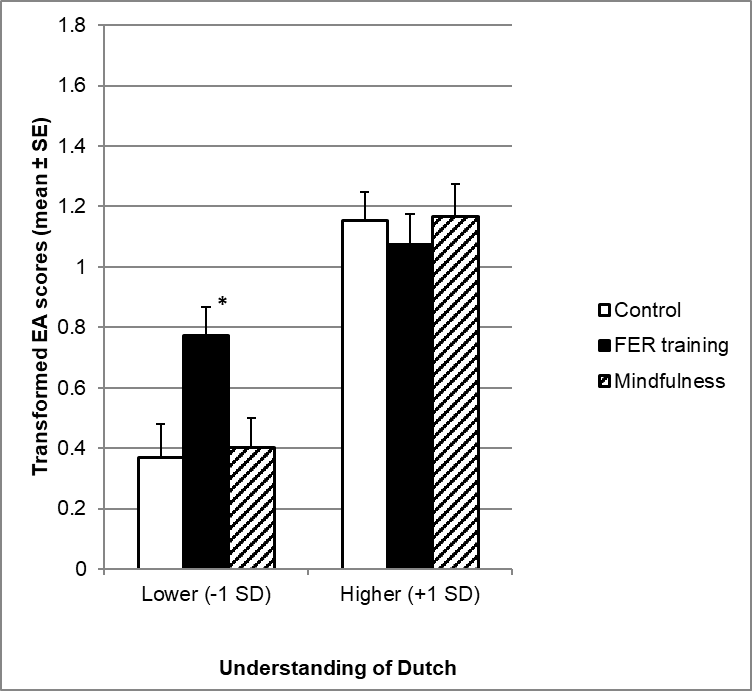
\includegraphics[scale=0.7]{media/image1.png}
	\caption{Alcohol-related picture examples (a, b), weapon-related picture examples (c, d), and neutral picture examples (e, f).}
\end{figure}
%%%%%%%%%%%%%%%%%%%% Figure/Image No: 1 Ends here %%%%%%%%%%%%%%%%%%%
\newpage

\subsection*{\hypertarget{A}{Appendix A}} 
\addcontentsline{toc}{subsection}{Appendix A}
\begin{Center}
Field of Study – Complete List
\end{Center}
%%%%%%%%%%%%%%%%%%%% Table No: 2 starts here %%%%%%%%%%%%%%%%%%%%
\begin{table}[H]
 			\centering
\begin{tabular}{p{1.6in}p{1.6in}} 
\hline
%row no:1
\multicolumn{1}{|p{1.3in}}{\Centering Field of study} & 
\multicolumn{1}{|p{1.3in}|}{\Centering \textit{n}} \\
\hhline{--}
%row no:2
\multicolumn{1}{|p{1.3in}}{Psychology} & 
\multicolumn{1}{|p{1.3in}|}{\Centering 38} \\
\hhline{--}
%row no:3
\multicolumn{1}{|p{1.3in}}{Biology} & 
\multicolumn{1}{|p{1.3in}|}{\Centering 4} \\
\hhline{--}
%row no:4
\multicolumn{1}{|p{1.3in}}{Languages} & 
\multicolumn{1}{|p{1.3in}|}{\Centering 3} \\
\hhline{--}
%row no:5
\multicolumn{1}{|p{1.3in}}{Education} & 
\multicolumn{1}{|p{1.3in}|}{\Centering 2} \\
\hhline{--}
%row no:6
\multicolumn{1}{|p{1.3in}}{Sociology} & 
\multicolumn{1}{|p{1.3in}|}{\Centering 2} \\
\hhline{--}
%row no:7
\multicolumn{1}{|p{1.3in}}{Physics} & 
\multicolumn{1}{|p{1.3in}|}{\Centering 1} \\
\hhline{--}
%row no:8
\multicolumn{1}{|p{1.3in}}{Politic Sciences} & 
\multicolumn{1}{|p{1.3in}|}{\Centering 1} \\
\hhline{--}
%row no:9
\multicolumn{1}{|p{1.3in}}{Biochemistry} & 
\multicolumn{1}{|p{1.3in}|}{\Centering 1} \\
\hhline{--}
%row no:10
\multicolumn{1}{|p{1.3in}}{History} & 
\multicolumn{1}{|p{1.3in}|}{\Centering 1} \\
\hhline{--}
%row no:11
\multicolumn{1}{|p{1.3in}}{English Literature} & 
\multicolumn{1}{|p{1.3in}|}{\Centering 1} \\
\hhline{--}
%row no:12
\multicolumn{1}{|p{1.3in}}{Mathematics} & 
\multicolumn{1}{|p{1.3in}|}{\Centering 1} \\
\hhline{--}
%row no:13
\multicolumn{1}{|p{1.3in}}{Finance} & 
\multicolumn{1}{|p{1.3in}|}{\Centering 1} \\
\hhline{--}
%row no:14
\multicolumn{1}{|p{1.3in}}{Arts Administrations} & 
\multicolumn{1}{|p{1.3in}|}{\Centering 1} \\
\hhline{--}
%row no:15
\multicolumn{1}{|p{1.3in}}{Sports Studies } & 
\multicolumn{1}{|p{1.3in}|}{\Centering 1} \\
\hhline{--}

\end{tabular}
 \end{table}

%%%%%%%%%%%%%%%%%%%% Table No: 2 ends here %%%%%%%%%%%%%%%%%%%%

\phantomsection
\addcontentsline{toc}{subsection}{Appendix B}
\subsection*{\hypertarget{B}{Appendix B}} 
\begin{Center}

\end{Center}
%%%%%%%%%%%%%%%%%%%% Figure/Image No: 2 starts here %%%%%%%%%%%%%%%%%%%%
\begin{figure}[H]
	\centering
	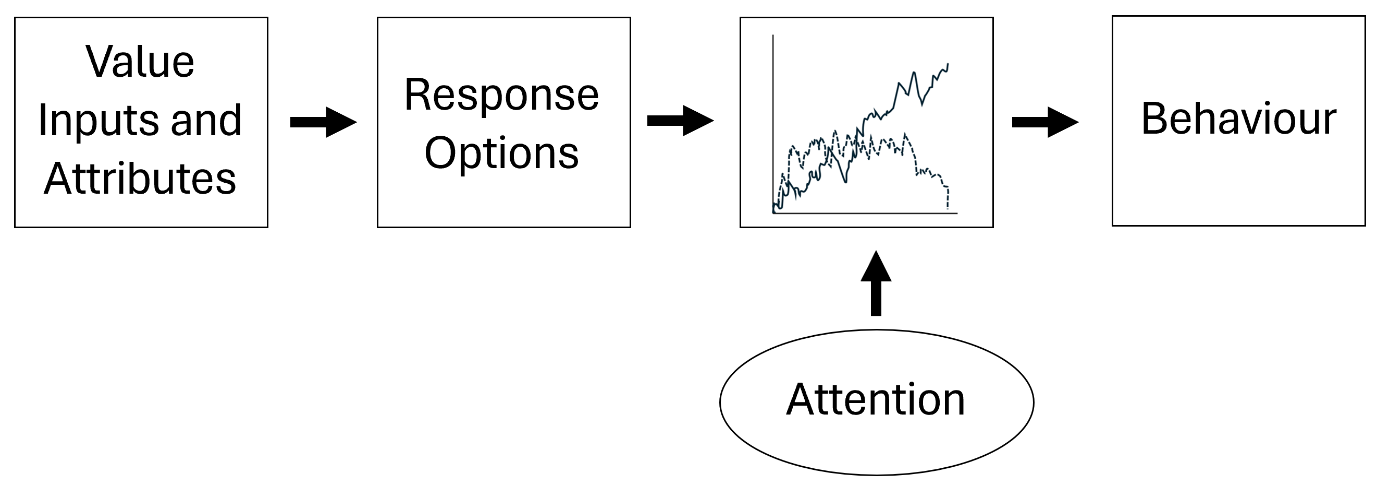
\includegraphics[width=5.54in,height=2.01in]{media/image2.png}
\end{figure}
%%%%%%%%%%%%%%%%%%%% Figure/Image No: 2 Ends here %%%%%%%%%%%%%%%%%%%%

\newpage
\phantomsection
\addcontentsline{toc}{subsection}{Appendix C}
\subsection*{\hypertarget{C}{Appendix C}}

\begin{Center}
German Extended Personal Attributes Questionnaire
\end{Center}

In general, I see \textbf{MEN} as being:



%%%%%%%%%%%%%%%%%%%% Table No: 3 starts here %%%%%%%%%%%%%%%%%%%%



%\setlength\extrarowheight{3pt}
\begin{longtable}{p{1.6in}p{0.2in}p{0.2in}p{0.2in}p{0.2in}p{0.2in}p{1.6in}}

\endfirsthead

\endfoot
\endlastfoot\hline
%row no:1
\multicolumn{1}{|p{1.6in}}{Not independent} & 
\multicolumn{1}{|p{0.2in}}{\textit{1}} & 
\multicolumn{1}{|p{0.2in}}{\textit{2}} & 
\multicolumn{1}{|p{0.2in}}{\textit{3}} & 
\multicolumn{1}{|p{0.2in}}{\textit{4}} & 
\multicolumn{1}{|p{0.2in}}{\textit{5}} & 
\multicolumn{1}{|p{1.6in}|}{Very independent} \\
\hhline{-------}
%row no:2
\multicolumn{1}{|p{1.6in}}{Very passive} & 
\multicolumn{1}{|p{0.2in}}{\textit{1}} & 
\multicolumn{1}{|p{0.2in}}{\textit{2}} & 
\multicolumn{1}{|p{0.2in}}{\textit{3}} & 
\multicolumn{1}{|p{0.2in}}{\textit{4}} & 
\multicolumn{1}{|p{0.2in}}{\textit{5}} & 
\multicolumn{1}{|p{1.6in}|}{Very active} \\
\hhline{-------}
%row no:3
\multicolumn{1}{|p{1.6in}}{Not competitive} & 
\multicolumn{1}{|p{0.2in}}{\textit{1}} & 
\multicolumn{1}{|p{0.2in}}{\textit{2}} & 
\multicolumn{1}{|p{0.2in}}{\textit{3}} & 
\multicolumn{1}{|p{0.2in}}{\textit{4}} & 
\multicolumn{1}{|p{0.2in}}{\textit{5}} & 
\multicolumn{1}{|p{1.6in}|}{Very competitive} \\
\hhline{-------}
%row no:4
\multicolumn{1}{|p{1.6in}}{Decisive} & 
\multicolumn{1}{|p{0.2in}}{\textit{1}} & 
\multicolumn{1}{|p{0.2in}}{\textit{2}} & 
\multicolumn{1}{|p{0.2in}}{\textit{3}} & 
\multicolumn{1}{|p{0.2in}}{\textit{4}} & 
\multicolumn{1}{|p{0.2in}}{\textit{5}} & 
\multicolumn{1}{|p{1.6in}|}{Not decisive} \\
\hhline{-------}
%row no:5
\multicolumn{1}{|p{1.6in}}{Gives up easily} & 
\multicolumn{1}{|p{0.2in}}{\textit{1}} & 
\multicolumn{1}{|p{0.2in}}{\textit{2}} & 
\multicolumn{1}{|p{0.2in}}{\textit{3}} & 
\multicolumn{1}{|p{0.2in}}{\textit{4}} & 
\multicolumn{1}{|p{0.2in}}{\textit{5}} & 
\multicolumn{1}{|p{1.6in}|}{Never gives up} \\
\hhline{-------}
%row no:6
\multicolumn{1}{|p{1.6in}}{Not self-confident} & 
\multicolumn{1}{|p{0.2in}}{\textit{1}} & 
\multicolumn{1}{|p{0.2in}}{\textit{2}} & 
\multicolumn{1}{|p{0.2in}}{\textit{3}} & 
\multicolumn{1}{|p{0.2in}}{\textit{4}} & 
\multicolumn{1}{|p{0.2in}}{\textit{5}} & 
\multicolumn{1}{|p{1.6in}|}{Self-confident} \\
\hhline{-------}
%row no:7
\multicolumn{1}{|p{1.6in}}{Feels inferior} & 
\multicolumn{1}{|p{0.2in}}{\textit{1}} & 
\multicolumn{1}{|p{0.2in}}{\textit{2}} & 
\multicolumn{1}{|p{0.2in}}{\textit{3}} & 
\multicolumn{1}{|p{0.2in}}{\textit{4}} & 
\multicolumn{1}{|p{0.2in}}{\textit{5}} & 
\multicolumn{1}{|p{1.6in}|}{Feels superior} \\
\hhline{-------}
%row no:8
\multicolumn{1}{|p{1.6in}}{Doesn’t stand up under pressure} & 
\multicolumn{1}{|p{0.2in}}{\textit{1}} & 
\multicolumn{1}{|p{0.2in}}{\textit{2}} & 
\multicolumn{1}{|p{0.2in}}{\textit{3}} & 
\multicolumn{1}{|p{0.2in}}{\textit{4}} & 
\multicolumn{1}{|p{0.2in}}{\textit{5}} & 
\multicolumn{1}{|p{1.6in}|}{Stands up under pressure} \\
\hhline{-------}
%row no:9
\multicolumn{1}{|p{1.6in}}{Not emotional} & 
\multicolumn{1}{|p{0.2in}}{\textit{1}} & 
\multicolumn{1}{|p{0.2in}}{\textit{2}} & 
\multicolumn{1}{|p{0.2in}}{\textit{3}} & 
\multicolumn{1}{|p{0.2in}}{\textit{4}} & 
\multicolumn{1}{|p{0.2in}}{\textit{5}} & 
\multicolumn{1}{|p{1.6in}|}{Very emotional} \\
\hhline{-------}
%row no:10
\multicolumn{1}{|p{1.6in}}{Devotes self to others} & 
\multicolumn{1}{|p{0.2in}}{\textit{1}} & 
\multicolumn{1}{|p{0.2in}}{\textit{2}} & 
\multicolumn{1}{|p{0.2in}}{\textit{3}} & 
\multicolumn{1}{|p{0.2in}}{\textit{4}} & 
\multicolumn{1}{|p{0.2in}}{\textit{5}} & 
\multicolumn{1}{|p{1.6in}|}{Doesn’t devote self to others} \\
\hhline{-------}
%row no:11
\multicolumn{1}{|p{1.6in}}{Very rough} & 
\multicolumn{1}{|p{0.2in}}{\textit{1}} & 
\multicolumn{1}{|p{0.2in}}{\textit{2}} & 
\multicolumn{1}{|p{0.2in}}{\textit{3}} & 
\multicolumn{1}{|p{0.2in}}{\textit{4}} & 
\multicolumn{1}{|p{0.2in}}{\textit{5}} & 
\multicolumn{1}{|p{1.6in}|}{Very gentle} \\
\hhline{-------}
%row no:12
\multicolumn{1}{|p{1.6in}}{Not helpful} & 
\multicolumn{1}{|p{0.2in}}{\textit{1}} & 
\multicolumn{1}{|p{0.2in}}{\textit{2}} & 
\multicolumn{1}{|p{0.2in}}{\textit{3}} & 
\multicolumn{1}{|p{0.2in}}{\textit{4}} & 
\multicolumn{1}{|p{0.2in}}{\textit{5}} & 
\multicolumn{1}{|p{1.6in}|}{Very helpful} \\
\hhline{-------}
%row no:13
\multicolumn{1}{|p{1.6in}}{Very unkind} & 
\multicolumn{1}{|p{0.2in}}{\textit{1}} & 
\multicolumn{1}{|p{0.2in}}{\textit{2}} & 
\multicolumn{1}{|p{0.2in}}{\textit{3}} & 
\multicolumn{1}{|p{0.2in}}{\textit{4}} & 
\multicolumn{1}{|p{0.2in}}{\textit{5}} & 
\multicolumn{1}{|p{1.6in}|}{Very kind} \\
\hhline{-------}
%row no:14
\multicolumn{1}{|p{1.6in}}{Not aware of feelings} & 
\multicolumn{1}{|p{0.2in}}{\textit{1}} & 
\multicolumn{1}{|p{0.2in}}{\textit{2}} & 
\multicolumn{1}{|p{0.2in}}{\textit{3}} & 
\multicolumn{1}{|p{0.2in}}{\textit{4}} & 
\multicolumn{1}{|p{0.2in}}{\textit{5}} & 
\multicolumn{1}{|p{1.6in}|}{Aware of feelings} \\
\hhline{-------}
%row no:15
\multicolumn{1}{|p{1.6in}}{Not understanding} & 
\multicolumn{1}{|p{0.2in}}{\textit{1}} & 
\multicolumn{1}{|p{0.2in}}{\textit{2}} & 
\multicolumn{1}{|p{0.2in}}{\textit{3}} & 
\multicolumn{1}{|p{0.2in}}{\textit{4}} & 
\multicolumn{1}{|p{0.2in}}{\textit{5}} & 
\multicolumn{1}{|p{1.6in}|}{Very understanding} \\
\hhline{-------}
%row no:16
\multicolumn{1}{|p{1.6in}}{Cold} & 
\multicolumn{1}{|p{0.2in}}{\textit{1}} & 
\multicolumn{1}{|p{0.2in}}{\textit{2}} & 
\multicolumn{1}{|p{0.2in}}{\textit{3}} & 
\multicolumn{1}{|p{0.2in}}{\textit{4}} & 
\multicolumn{1}{|p{0.2in}}{\textit{5}} & 
\multicolumn{1}{|p{1.6in}|}{Warm} \\
\hhline{-------}

\end{longtable}

%%%%%%%%%%%%%%%%%%%% Table No: 3 ends here %%%%%%%%%%%%%%%%%%%%



In general, I see \textbf{WOMEN} as being:



%%%%%%%%%%%%%%%%%%%% Table No: 4 starts here %%%%%%%%%%%%%%%%%%%%



%\setlength\extrarowheight{3pt}
\begin{longtable}{p{1.6in}p{0.2in}p{0.2in}p{0.2in}p{0.2in}p{0.2in}p{1.6in}}

\endfirsthead

\endfoot
\endlastfoot\hline
%row no:1
\multicolumn{1}{|p{1.6in}}{Not independent} & 
\multicolumn{1}{|p{0.2in}}{\textit{1}} & 
\multicolumn{1}{|p{0.2in}}{\textit{2}} & 
\multicolumn{1}{|p{0.2in}}{\textit{3}} & 
\multicolumn{1}{|p{0.2in}}{\textit{4}} & 
\multicolumn{1}{|p{0.2in}}{\textit{5}} & 
\multicolumn{1}{|p{1.6in}|}{Very independent} \\
\hhline{-------}
%row no:2
\multicolumn{1}{|p{1.6in}}{Very passive} & 
\multicolumn{1}{|p{0.2in}}{\textit{1}} & 
\multicolumn{1}{|p{0.2in}}{\textit{2}} & 
\multicolumn{1}{|p{0.2in}}{\textit{3}} & 
\multicolumn{1}{|p{0.2in}}{\textit{4}} & 
\multicolumn{1}{|p{0.2in}}{\textit{5}} & 
\multicolumn{1}{|p{1.6in}|}{Very active} \\
\hhline{-------}
%row no:3
\multicolumn{1}{|p{1.6in}}{Not competitive} & 
\multicolumn{1}{|p{0.2in}}{\textit{1}} & 
\multicolumn{1}{|p{0.2in}}{\textit{2}} & 
\multicolumn{1}{|p{0.2in}}{\textit{3}} & 
\multicolumn{1}{|p{0.2in}}{\textit{4}} & 
\multicolumn{1}{|p{0.2in}}{\textit{5}} & 
\multicolumn{1}{|p{1.6in}|}{Very competitive} \\
\hhline{-------}
%row no:4
\multicolumn{1}{|p{1.6in}}{Decisive} & 
\multicolumn{1}{|p{0.2in}}{\textit{1}} & 
\multicolumn{1}{|p{0.2in}}{\textit{2}} & 
\multicolumn{1}{|p{0.2in}}{\textit{3}} & 
\multicolumn{1}{|p{0.2in}}{\textit{4}} & 
\multicolumn{1}{|p{0.2in}}{\textit{5}} & 
\multicolumn{1}{|p{1.6in}|}{Not decisive} \\
\hhline{-------}
%row no:5
\multicolumn{1}{|p{1.6in}}{Gives up easily} & 
\multicolumn{1}{|p{0.2in}}{\textit{1}} & 
\multicolumn{1}{|p{0.2in}}{\textit{2}} & 
\multicolumn{1}{|p{0.2in}}{\textit{3}} & 
\multicolumn{1}{|p{0.2in}}{\textit{4}} & 
\multicolumn{1}{|p{0.2in}}{\textit{5}} & 
\multicolumn{1}{|p{1.6in}|}{Never gives up} \\
\hhline{-------}
%row no:6
\multicolumn{1}{|p{1.6in}}{Not self-confident} & 
\multicolumn{1}{|p{0.2in}}{\textit{1}} & 
\multicolumn{1}{|p{0.2in}}{\textit{2}} & 
\multicolumn{1}{|p{0.2in}}{\textit{3}} & 
\multicolumn{1}{|p{0.2in}}{\textit{4}} & 
\multicolumn{1}{|p{0.2in}}{\textit{5}} & 
\multicolumn{1}{|p{1.6in}|}{Self-confident} \\
\hhline{-------}
%row no:7
\multicolumn{1}{|p{1.6in}}{Feels inferior} & 
\multicolumn{1}{|p{0.2in}}{\textit{1}} & 
\multicolumn{1}{|p{0.2in}}{\textit{2}} & 
\multicolumn{1}{|p{0.2in}}{\textit{3}} & 
\multicolumn{1}{|p{0.2in}}{\textit{4}} & 
\multicolumn{1}{|p{0.2in}}{\textit{5}} & 
\multicolumn{1}{|p{1.6in}|}{Feels superior} \\
\hhline{-------}
%row no:8
\multicolumn{1}{|p{1.6in}}{Doesn’t stand up under pressure} & 
\multicolumn{1}{|p{0.2in}}{\textit{1}} & 
\multicolumn{1}{|p{0.2in}}{\textit{2}} & 
\multicolumn{1}{|p{0.2in}}{\textit{3}} & 
\multicolumn{1}{|p{0.2in}}{\textit{4}} & 
\multicolumn{1}{|p{0.2in}}{\textit{5}} & 
\multicolumn{1}{|p{1.6in}|}{Stands up under pressure} \\
\hhline{-------}
%row no:9
\multicolumn{1}{|p{1.6in}}{Not emotional} & 
\multicolumn{1}{|p{0.2in}}{\textit{1}} & 
\multicolumn{1}{|p{0.2in}}{\textit{2}} & 
\multicolumn{1}{|p{0.2in}}{\textit{3}} & 
\multicolumn{1}{|p{0.2in}}{\textit{4}} & 
\multicolumn{1}{|p{0.2in}}{\textit{5}} & 
\multicolumn{1}{|p{1.6in}|}{Very emotional} \\
\hhline{-------}
%row no:10
\multicolumn{1}{|p{1.6in}}{Devotes self to others} & 
\multicolumn{1}{|p{0.2in}}{\textit{1}} & 
\multicolumn{1}{|p{0.2in}}{\textit{2}} & 
\multicolumn{1}{|p{0.2in}}{\textit{3}} & 
\multicolumn{1}{|p{0.2in}}{\textit{4}} & 
\multicolumn{1}{|p{0.2in}}{\textit{5}} & 
\multicolumn{1}{|p{1.6in}|}{Doesn’t devote self to others} \\
\hhline{-------}
%row no:11
\multicolumn{1}{|p{1.6in}}{Very rough} & 
\multicolumn{1}{|p{0.2in}}{\textit{1}} & 
\multicolumn{1}{|p{0.2in}}{\textit{2}} & 
\multicolumn{1}{|p{0.2in}}{\textit{3}} & 
\multicolumn{1}{|p{0.2in}}{\textit{4}} & 
\multicolumn{1}{|p{0.2in}}{\textit{5}} & 
\multicolumn{1}{|p{1.6in}|}{Very gentle} \\
\hhline{-------}
%row no:12
\multicolumn{1}{|p{1.6in}}{Not helpful} & 
\multicolumn{1}{|p{0.2in}}{\textit{1}} & 
\multicolumn{1}{|p{0.2in}}{\textit{2}} & 
\multicolumn{1}{|p{0.2in}}{\textit{3}} & 
\multicolumn{1}{|p{0.2in}}{\textit{4}} & 
\multicolumn{1}{|p{0.2in}}{\textit{5}} & 
\multicolumn{1}{|p{1.6in}|}{Very helpful} \\
\hhline{-------}
%row no:13
\multicolumn{1}{|p{1.6in}}{Very unkind} & 
\multicolumn{1}{|p{0.2in}}{\textit{1}} & 
\multicolumn{1}{|p{0.2in}}{\textit{2}} & 
\multicolumn{1}{|p{0.2in}}{\textit{3}} & 
\multicolumn{1}{|p{0.2in}}{\textit{4}} & 
\multicolumn{1}{|p{0.2in}}{\textit{5}} & 
\multicolumn{1}{|p{1.6in}|}{Very kind} \\
\hhline{-------}
%row no:14
\multicolumn{1}{|p{1.6in}}{Not aware of feelings} & 
\multicolumn{1}{|p{0.2in}}{\textit{1}} & 
\multicolumn{1}{|p{0.2in}}{\textit{2}} & 
\multicolumn{1}{|p{0.2in}}{\textit{3}} & 
\multicolumn{1}{|p{0.2in}}{\textit{4}} & 
\multicolumn{1}{|p{0.2in}}{\textit{5}} & 
\multicolumn{1}{|p{1.6in}|}{Aware of feelings} \\
\hhline{-------}
%row no:15
\multicolumn{1}{|p{1.6in}}{Not understanding} & 
\multicolumn{1}{|p{0.2in}}{\textit{1}} & 
\multicolumn{1}{|p{0.2in}}{\textit{2}} & 
\multicolumn{1}{|p{0.2in}}{\textit{3}} & 
\multicolumn{1}{|p{0.2in}}{\textit{4}} & 
\multicolumn{1}{|p{0.2in}}{\textit{5}} & 
\multicolumn{1}{|p{1.6in}|}{Very understanding} \\
\hhline{-------}
%row no:16
\multicolumn{1}{|p{1.6in}}{Cold} & 
\multicolumn{1}{|p{0.2in}}{\textit{1}} & 
\multicolumn{1}{|p{0.2in}}{\textit{2}} & 
\multicolumn{1}{|p{0.2in}}{\textit{3}} & 
\multicolumn{1}{|p{0.2in}}{\textit{4}} & 
\multicolumn{1}{|p{0.2in}}{\textit{5}} & 
\multicolumn{1}{|p{1.6in}|}{Warm} \\
\hhline{-------}
\end{longtable}
%%%%%%%%%%%%%%%%%%%% Table No: 4 ends here %%%%%%%%%%%%%%%%%%%%
\newpage
\phantomsection
\addcontentsline{toc}{subsection}{Appendix D}
\subsection*{\hypertarget{D}{Appendix D}}

\begin{Center}
Target Word Type – Complete List
\end{Center}

%%%%%%%%%%%%%%%%%%%% Table No: 5 starts here %%%%%%%%%%%%%%%%%%%%


\begin{table}[H]
 			\centering
\begin{tabular}{p{0.9in}p{0.9in}p{0.9in}}
%row no:1
\multicolumn{1}{p{0.9in}}{Neutral Words} & 
\multicolumn{1}{p{0.9in}}{Aggressive Words} & 
\multicolumn{1}{p{0.9in}}{Nonwords} \\
\hhline{~~~}
%row no:2
\multicolumn{1}{p{0.9in}}{Glide \newline Suggest \newline  Observe\newline  Vanish\newline  Move\newline  Narrate\newline  Imagine\newline  Ignored\newline  Improve\newline  Joked\newline  Read\newline  Leave\newline  Listen\newline  Transfer\newline  Reported} & 
\multicolumn{1}{p{0.9in}}{Touching\newline Incest\newline  Coercion\newline  Molest\newline  Sodomy\newline  Harassment\newline  Grope\newline  Rape\newline  Prey\newline  Perversion\newline  Abuse\newline  Violated\newline  Choke\newline  Stalking\newline   Roofies} & 
\multicolumn{1}{p{0.9in}}{Sarf\newline  Philst\newline  Wenct\newline  Jork\newline  Atand\newline  Kesh\newline  Morpe\newline  Farn\newline  Lerf\newline  Chib\newline  Dephs\newline  Anage\newline  Steay\newline  Omoga\newline  Benct} \\
\hhline{~~~}

\end{tabular}
\end{table}


%%%%%%%%%%%%%%%%%%%% Table No: 5 ends here %%%%%%%%%%%%%%%%%%%%
\printbibliography


\end{document} 